\documentclass[10pt, a4paper,english,spanish]{article}
%\documentclass[10pt,a4paper]{article}
\usepackage[utf8]{inputenc} % para poder usar tildes en archivos UTF-8
\usepackage[spanish]{babel} % para que comandos como \today den el resultado en castellano
\usepackage[conEntregas]{caratula}
\usepackage{fullpage} %small margins
\usepackage[parfill]{parskip} %genera saltos entre parrafos
\usepackage{color}
\definecolor{gray}{gray}{0.35}
\usepackage{listings}
\usepackage{enumitem}
\usepackage{soul}
\usepackage{amsmath} %big brackets
\usepackage[pdftex]{graphicx}
\lstset{
    numbers=left,
    breaklines=true,
    tabsize=2,
    basicstyle=\ttfamily\color{gray},
}
\setlength{\parindent}{8pt}
\usepackage{mathtools}
\usepackage[margin=50pt]{geometry}
\usepackage{amsfonts}
\usepackage{flafter}
\usepackage{multicol}
\usepackage{caption}
\usepackage{subcaption}
\usepackage{graphicx}
\setlength{\parindent}{0pt} %remueve indent

%paquete para setear colores a las tablas para graficar registros
\usepackage{xcolor,colortbl}
%define de colores
\definecolor{Orange}{rgb}{1, 0.64, 0}
\definecolor{Green}{rgb}{0.32,1,0.62}
%\definecolor{Purple}{rgb}{0.44,0.20,0.81}
%define de columnas
\newcolumntype{o}{>{\columncolor{Orange}}c}
\newcolumntype{g}{>{\columncolor{Green}}c}
%\newcolumntype{p}{>{\columncolor{Purple}}c}
%holi
\begin{document}

\materia{Organización del Computador II}
\submateria{Trabajo Práctico Nro. 2}
\titulo{Filtros de imágenes - Grupo: SnakeII/Nokia1100}
\fecha{\today}
\integrante{Pablo Gomez}{156/13}{mago-1986@hotmail.com}
\integrante{Lucia Parral}{162/13}{luciaparral@gmail.com}
\integrante{Petr Romachov}{412/13}{promachov@gmail.com}
\maketitle
\newpage

\tableofcontents

\newpage
\section{Introducción}
En este trabajo práctico se busca experimentar con el procesamiento con instrucciones SIMD que operan con múltiples datos simultáneamente.\\ 
Con este fin, desarrollamos distintas implementaciones de los filtros Blur, Merge y HSL sobre imágenes y evaluamos su rendimiento.\\
\subsection{Sobre la experimentación}
Realizamos las experimentaciones para los tres filtros con sus respectivas implementaciones de la manera detallada a continuación.\\
Para realizar casos de tests exhaustivos, utilizamos imágenes de distintos tamaños y tipos.
Tomamos imágenes de colores constantes (es decir, imágenes totalmente blancas, azules, verdes, rojas y negras), imágenes que tienden a estos colores e imágenes mixtas.
Cada una de estas imágenes las procesamos en los tamaños 40x40 (1600 píxeles), 300x300 (90000 píxeles) y 600x600 (360000 píxeles), ya que nos pareció una variación razonable para mostrar la performance de las distintas implementaciones de los filtros.\\
Para cada filtro y cada implementación, calculamos la cantidad de ciclos de clock que transcurren en las instrucciones que procesan la imagen (obviando la carga de la misma y el guardado de datos). Para medir los ciclos de clock usamos las funciones provistas por la cátedra en el archivo rdtsc.h. 
Teniendo en cuenta que existen problemáticas al momento de conocer el tiempo de ejecución real de los programas, ya que la ejecución puede ser interrumpida por el scheduler para realizar un cambio de contexto o bien que los procesadores varían la frecuencia de reloj, ideamos la siguiente metodología para medir la cantidad de ciclos de clock de nuestras implementaciones: para cada test entonces, realizamos 100 repeticiones, tomando el promedio de los resultados obtenidos.\\ Luego, descartamos el 10\% de los peores casos. Una vez hecho esto, calculamos el desvío estándar del 90\% de los casos restantes. De esta forma, obtuvimos un resultado promedio, y sumando y restando a este valor el desvío estándar, el resultado esperado en mejor y peor caso. Así mismo, el desvío estándar también nos sirve como indicador de qué tan precisas fueron las mediciones.\\
Además, compilamos las implementaciones de C provistas por la cátedra con el parámetro de compilación -O3, que aseguraba la versión más optimizada del código, para poder acercarnos a la mejor ejecución posible de dichas implementaciones.\\

%TODO: Calcular o chamuyar el desvío estándar en las mediciones y hablar un poco de eso luego.

Cabe destacar que la computadora en la que realizamos las experimentaciones cuenta con las siguientes especificaciones técnicas:\\
%TODO: Agregar características técnicas de la computadora del Mago

Para experimentar acerca de si variaba el rendimiento de una implementación en función del tipo de imagen testeado elaboramos la siguiente estrategia. Agrupamos los distintos tipos de imágenes con los que contábamos como casos de prueba, descritos en la introducción del apartado de experimentación, y tomamos el promedio de tiempos de ejecución (tomando el 10\% peor como outliers) para cada subgrupo. Luego, tomando los promedios de cada tipo de imagen como el representante de dicho tipo, calculamos el desvío estándar entre todos los representantes. Una vez calculado el desvío estándar, lo dividimos por el promedio y multiplicamos por 100 para tener un “porcentaje de desviación”. De esta forma, un porcentaje elevado significa que los representantes de cada tipo de imagen difieren significativamente, mientras que un porcentaje pequeño, que todos los representantes estan cercanos al promedio y por lo tanto, las mediciones dentro de todos los tipos se mantiene estable.\\

Por último, tomamos como decisión para una mayor claridad en los gráficos, el utilizar escala logarítmica para representar los ciclos de clock, ya que de no hacerlo, se perdía claridad y representatividad en los mismos. De cualquier manera, en cada gráfico figurará qué tipo de escala está utilizando, y cualquier otra información relevante.
A continuación, describiremos para cada filtro su desarrolo, los resultados obtenidos y el análisis comparativo en relación con las implementaciones que realizamos y otras posibles.\\\\\\\\\\\\\\\\\\

% \begin{figure}[ht]
% \centering
% 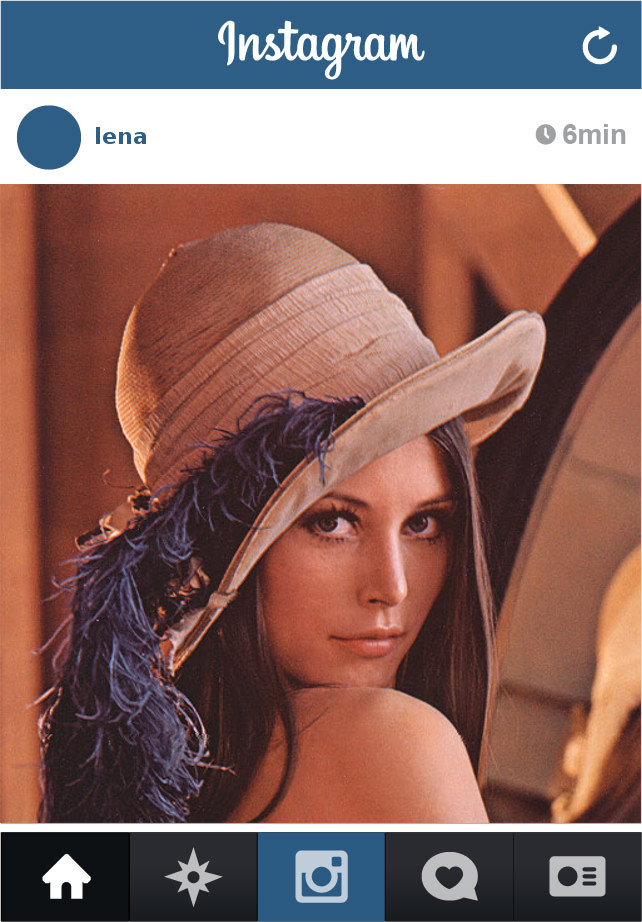
\includegraphics[width=90mm]{introduccion/lena_instagram.jpg}
% %\caption{A simple caption \label{overflow}}
% \end{figure}


\newpage
% Comienzo Blur
\section{Blur}
\subsection{Introducción}
\textit{Blur} es un filtro que suaviza una imagen. Le asigna a cada pixel el promedio con sus pixeles vecinos.\\ Es decir:

\begin{verbatim}
  m[j][i][k] = (m[j-1][i-1][k] + m[j-1][i][k] + m[j-1][i+1][k] + 
              m[j] [i-1][k] + m[j] [i][k] + m[j] [i+1][k] + 
              m[j+1][i-1][k] + m[j+1][i][k] + m[j+1][i+1][k] ) / 9
\end{verbatim}

De esta forma, la salida es la imagen en donde para cada pixel, se realizó el "suavizado" según el cálculo anterior.

\subsection{Pseudocódigo en C}

El pseudocódigo para una iteración del ciclo de la implementación de C provista por la cátedra es:

\begin{lstlisting}

//TODO: Mejorar este pseudocodigo

for(iw=0;iw<(int)w;iw++) {
    for(ii=0;ii<4;ii++) {
      m_row_1[iw][ii] = m[0][iw][ii];
    }
  }
  for(ih=1;ih<(int)h-1;ih++) {
    m_tmp = m_row_0;
    m_row_0 = m_row_1;
    m_row_1 = m_tmp;
    for(iw=0;iw<(int)w;iw++) {
      for(ii=0;ii<4;ii++) {
        m_row_1[iw][ii] = m[ih][iw][ii];
      }
    }
    for(iw=1;iw<(int)w-1;iw++) {
      for(ii=0;ii<4;ii++) {
        m[ih][iw][ii] = ( 
          (int)m_row_0[iw-1][ii] + (int)m_row_0[iw][ii] + (int)m_row_0[iw+1][ii] +
          (int)m_row_1[iw-1][ii] + (int)m_row_1[iw][ii] + (int)m_row_1[iw+1][ii] +
          (int)m[ih+1][iw-1][ii] + (int)m[ih+1][iw][ii] + (int)m[ih+1][iw+1][ii] ) / 9;
      }
    }
  }

\end{lstlisting}

\subsection{Implementación 1 en ASM}
La primera implementación consiste en procesar de a un pixel por iteración.\\

La implementación comienza pidiendo memoria a través de \textit{malloc}, igual que C, para copiar dos filas de la imagen a procesar.\\
Esto se hace debido a que de no hacerlo se presenta el siguiente problema: dado un pixel X que acaba de ser blureado, el pixel siguiente no puede tomar el valor de X para calcular el promedio de croma ya que este perdió su valor original. Notar que tampoco puede leer los de la fila anterior recién blureada, por el mismo problema; los únicos que puede leer son los de la fila 'siguiente', que aún no fue blureada. Entonces, necesitamos de 2 espacios de memoria para 'backupearlas', y poder leer de allí los valores originales.\\

Para la primera vez, se backupean las dos primeras filas y luego se van copiando en el ciclo de ejecución las 2 filas necesarias para cada fila que se bluree.Es por esta razón, que se comienza a blurear desde la segunda fila y no desde la primera.\\

En cuanto al ciclo en sí, levanta de a 4 píxeles de tres lugares distintos:
\begin{enumerate}
\item De uno de los 2 espacios de memoria mencionados, que contiene la fila anterior ya blureada.
\item Del otro de los 2 espacios de memoria mencionados, que contiene la fila que se está blureando actualmente.
\item De la fila siguiente que aún no fue blureada. (Como no fue blureada, sus componentes de croma contienen el valor original y pueden leerse). \\
\end{enumerate}
A pesar de que se levantan de a cuatro píxeles, solo usamos 3 de ellos, ya que necesitamos 3 de cada uno para conseguir el promedio dado por el pseudocódigo provisto en el enunciado del TP.\\

Una cuestión importante es que los 4 píxeles que levantamos de la imagen original (de la fila que aún no fue blureada) son tomados 'defasados' 1 píxel a la izquierda, con el fin de no 'salirnos' de la imagen en el cálculo del último pixel. Notar que levantar defasados a la izquierda un pixel no hace que no accedamos a memoria que no es nuestra, ya que el pixel 'fuera' de la imagen que estamos pidiendo en la primer iteración, en realidad no está fuera de la imagen, ya que la iteración comienza en la segunda fila, por ende, ese pixel mencionado, pertenece a la primer fila, que es memoria accesible.

A continuación, shifteamos 1 pixel a derecha para subsanar lo recientemente explicado y tener los 3 píxeles que utilizaremos en la parte menos significativa de los xmm.

Eso hace que en este punto tengamos, en los 96 bits (3/4 de 128) menos significativos 3 xmms distintos, los 9 valores que necesitamos para blurear.

Una vez con los 9 píxeles guardados en registros xmm, calculamos el promedio y lo aplicamos al pixel correspondiente. Para hacer esto tuvimos que 'unpackear' los píxeles obtenidos para poder trabajar con las cromas separadas, y para poder realizar sumas con confianza, ya que si bien cada croma ocupa 8 bits (1 byte), sumar las 9 cromas de los 9 píxeles podría necesitar un tamaño mayor al de 8 bits. Para lograr un rango seguro, debimos 'unpackear' hasta dwords.

Luego, pasamos a floats las sumas para poder dividir, realizamos la division por 9 y volvimos a pasarlos a enteros para así finalizar el 'blureo' del píxel actual.

Finalmente, avanzamos un píxel y volvemos a iterar.\\

\subsection{Implementación 2 en ASM}
La implementación ASM2 realiza casi lo mismo que la ASM1 pero con la variación de que en vez de escribir en memoria 1 solo pixel, escribe 2, ya que el cálculo realizado es el mismo. Luego como escribió 2 píxeles, avanza dos en la fila y realiza el mismo procedimiento. Teoricamente esta implementación debería realizar la mitad de ciclos de iteración ya que puede calcular 2 pixeles al mismo tiempo en vez de a 1, es decir.


\subsection{Resultados}
A continuación, detallamos los resultados obtenidos a través de la experimentación con las distintas implementaciones en C y Assembler para este filtro y las conclusiones a las que llegamos tras el estudio de los mismos.\\
Tener en cuenta que el porcentaje de desvío estándard para cada implementación de este filtro resultó ser de:
\begin{tabular}{| l | l |}
\hline
Implementación & Porcentaje de Desvío Estándard \\
Blur C  & $+/- 4.8\%$\\
Blur ASM1 &   $+/- 13.8\%$\\
Blur ASM2 & $+/- 12\%$\\
\hline
\end{tabular}

Estos porcentajes representan que, para cada medición de cantidad de ciclos de clock de ejecución de una implementación dada de este filtro, tras descartar el 10\% de las peores mediciones, y tomar el promedio entre el 90\% de las mediciones restantes, el error varía entre +/- dicho porcentaje. Por ejemplo, dada la ejecución siguiente:\\

\begin{verbatim}
c blur image_1_40x40.bmp salida.bmp
\end{verbatim}
Sobre las 100 repeticiones realizadas, tras descartar el 10\% de las peores, quedan 90 mediciones sobre las cuales el promedio calculado fue 319538 con margen de error de +/-3\%.\\
Las siguientes son las tablas resultantes de tomar el promedio de todos los tiempos medidos para imágenes tendientes a un mismo color, para los distintos tamaños evaluados, según se detalla en la introducción.\\

\begin{tabular}{| l | l | l | l | l |}
\hline
Implementación & Color & 1600 píxeles & 90000 píxeles & 360000 píxeles\\
\hline
Blur ASM1 & azul & 29333.87 & 1389083.47&  5590953.07\\ 
\hline
Blur ASM1 & blanco & 28953.00&  1319802.00 & 5539200.67\\ 
\hline
Blur ASM1 & mixto & 28765.56  &1369988.44  & 5712646.67\\ 
\hline
Blur ASM1 & negro & 28342.25  &1367054.50  & 5607272.25\\
\hline
Blur ASM1 & rojo & 28703.00  &1370567.00  & 5651159.63\\
\hline
Blur ASM1 & verde & 28895.03  &1363316.78  & 5635944.92\\ 
\hline
Promedio & &  28895.03  &1363316.78 & 5635944.92\\
\hline
Desvio estándard  && 373.53  &23102.01 &  69973.61\\
\hline
Porcentaje de desviación  && 1.29\%& 1.69\%& 1.24\%\\
\hline
\end{tabular}

\begin{tabular}{| l | l | l | l | l |}
\hline
Implementación & Color & 1600 píxeles & 90000 píxeles & 360000 píxeles\\
\hline
Blur ASM2 & azul & 17992.73 &  750119.40&  3141036.87\\ 
\hline
Blur ASM2 & blanco & 18219.67  & 770902.67 & 3104900.00\\ 
\hline
Blur ASM2 & mixto &  17272 & 752688.88 & 3157686.11\\ 
\hline
Blur ASM2 & negro & 18470.50  & 776735.75 & 3127282.25\\
\hline
Blur ASM2 & rojo & 17351.25 &  732310.25 & 3165519.38\\
\hline
Blur ASM2 & verde & 17755.25 & 765754.75 & 3170724.75\\ 
\hline
Promedio & &  17843.57  & 758085.28 & 3144524.89\\
\hline
Desvio estándard  && 476.15  & 16296.47  & 25219.14\\
\hline
Porcentaje de desviación  && 2.67\% & 2.15\% & 0.80\%\\
\hline
\end{tabular}

\begin{tabular}{| l | l | l | l | l |}
\hline
Implementación & Color & 1600 píxeles & 90000 píxeles & 360000 píxeles\\
\hline
Blur C & azul & 306557.40 & 14795203.80 & 59272448.00\\ 
\hline
Blur C & blanco & 272834.33 & 15306523.00 & 57771410.67\\ 
\hline
Blur C & mixto &  297517.11 & 14445272.00 & 57421879.56\\ 
\hline
Blur C & negro & 331603.75 & 16997981.00 & 59230171.00\\
\hline
Blur C & rojo & 286341.13 & 14904426.13 & 57154062.00\\
\hline
Blur C & verde & 287608.75 & 14182027.25 & 58559933.00\\ 
\hline
Promedio & &  297077.08 & 15105238.86 & 58234984.04\\
\hline
Desvio estándard  && 20370.47  & 1004720.01 & 918341.11\\
\hline
Porcentaje de desviación  && 6.86\% & 6.65\% & 1.58\%\\
\hline
\end{tabular}

Finalmente, tomando los promedios para todos los tipos de imágenes para cada implementación y tamaño, logramos el siguiente gráfico que permite evaluar comparativamente la performance de las distintas implementaciones para los distintos tamaños.

\begin{tabular}{| l | l | l | l|}
\hline
Implementación  & 1600 píxeles & 90000 píxeles & 360000 píxeles\\
\hline
Blur ASM1  & 17843.57 & 758085.28 & 2618274.34\\
\hline
Blur ASM2  & 28895.03 & 1363316.78 & 5635944.92\\
\hline
Blur C & 297077.08 & 15105238.86 & 58234984.04\\
\hline
\end{tabular}

\begin{figure}[ht]
\centering
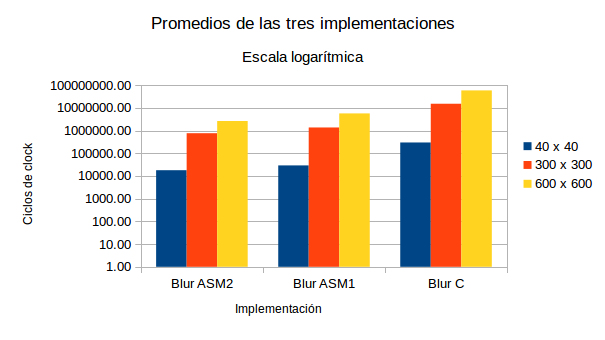
\includegraphics[width=90mm]{blur/graficoBlur.png}
%\caption{A simple caption \label{overflow}}
\end{figure}

Para evaluar si había diferencias en imágenes de un color constante, realizamos los mismos experimentos en este set de caso de pruebas, compuesto con imágenes puramente verdes, azules, rojas, blancas y negras. A continuación, las tablas con resultados de estos experimentos, junto con el gráfico resultante.\\

\begin{tabular}{| l | l | l | l | l |}
\hline
Implementación & Color & 1600 píxeles & 90000 píxeles & 360000 píxeles\\
\hline
Blur ASM1 & Uniforme Blanca & 25158.00 & 1415168.00 & 5707722.00\\ 
\hline
Blur ASM1 & Uniforme Negra & 25008.00 & 1417360.00 & 5821901.00\\ 
\hline
Blur ASM1 & Uniforme Roja & 23542.00 & 1429305.00 & 5522346.00\\ 
\hline
Blur ASM1 & Uniforme Verde & 24259.00 & 1424455.00 & 5663435.00\\
\hline
Blur ASM1 & Uniforme Azul & 23421.00 & 1384261.00 & 5752064.00\\
\hline
Promedio & &  24277.60 & 1414109.80 & 5693493.60\\
\hline
Desvio estándard  &&  803.71 & 17610.73 & 112156.61\\
\hline
Porcentaje de desviación  &&  3.31\% & 1.25\% & 1.97\%\\
\hline
\end{tabular}


\begin{tabular}{| l | l | l | l | l |}
\hline
Implementación & Color & 1600 píxeles & 90000 píxeles & 360000 píxeles\\
\hline
Blur ASM2 & Uniforme Blanca & 13297.00 & 769413.00 & 3180362.00\\ 
\hline
Blur ASM2 & Uniforme Negra & 15364.00 & 777099.00 & 3055456.00\\ 
\hline
Blur ASM2 & Uniforme Roja & 14031.00 & 776847.00 & 3132449.00\\ 
\hline
Blur ASM2 & Uniforme Verde & 16060.00 & 743686.00 & 3191171.00\\
\hline
Blur ASM2 & Uniforme Azul & 14278.00 & 778483.00 & 3159916.00\\
\hline
Promedio & &   14606.00 & 769105.60 & 3143870.80\\
\hline
Desvio estándard  &&  1100.04 & 14645.90 & 54254.03\\
\hline
Porcentaje de desviación  &&   7.53\% & 1.90\% & 1.73\%\\
\hline
\end{tabular}

\begin{tabular}{| l | l | l | l | l |}
\hline
Implementación & Color & 1600 píxeles & 90000 píxeles & 360000 píxeles\\
\hline
Blur C & Uniforme Blanca & 306566.00 & 14236027.00 & 56984192.00\\ 
\hline
Blur C & Uniforme Negra & 303997.00 & 14469139.00 & 56284032.00\\ 
\hline
Blur C & Uniforme Roja & 300376.00 & 14622681.00 & 55996348.00\\ 
\hline
Blur C & Uniforme Verde & 295486.00 & 14840694.00 & 56661072.00\\
\hline
Blur C & Uniforme Azul & 300286.00 & 14917069.00 & 55887204.00\\
\hline
Promedio & &   301342.20 & 14617122.00 & 56362569.60\\
\hline
Desvio estándard  &&  4203.58 & 277090.20 & 458742.02\\
\hline
Porcentaje de desviación  &&   1.39\% & 1.90\% & 0.81\%\\
\hline
\end{tabular}

A partir de esta información, logramos la siguiente tabla que recopila los promedios y nos permite realizar un gráfico comparativo de implementaciones según tamaño.\\



\begin{tabular}{| l | l | l | l|}
\hline
Implementación  & 1600 píxeles & 90000 píxeles & 360000 píxeles\\
\hline
Blur ASM1  & 24277.6 & 1414109.8 & 5693493.6\\
\hline
Blur ASM2  &  14606 & 769105.6 & 3143870.8\\
\hline
Blur C & 301342.2 & 14617122 & 56362569.6\\
\hline
\end{tabular}

\begin{figure}[ht]
\centering
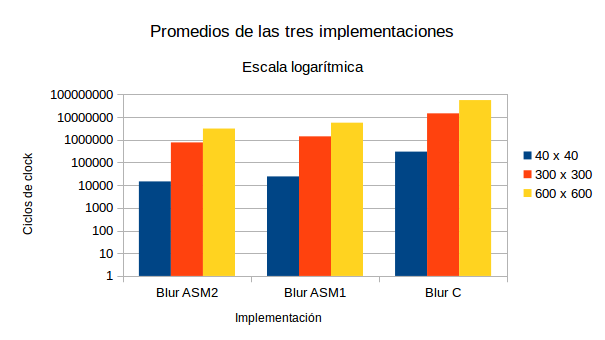
\includegraphics[width=90mm]{blur/graficoBlur_cte.png}
%\caption{A simple caption \label{overflow}}
\end{figure}

\subsubsection{Algunas conclusiones}
Dentro de cada implementación, vemos que el tiempo de ejecución aumenta a medida que aumenta el tamaño de las imágenes de prueba, lo cual era en cierto sentido lo que nos indicaba nuestro intuición que iba a suceder.\\
Así mismo, la implementación más performante resultó ser ASM2.\\
Este resultado no pareciera depender de la cantidad de instrucciones, dado que ambas implementaciones de Assembler poseen una cantidad muy similar de las mismas. 
%todo: me parece que tiene que ver con los accesos a memoria, chequear.
También pudimos corroborar, que para este filtro, el tipo de imagen elegido no afectaba en la performance de la implementación, ya que los porcentajes de desvío son muy pequeños, lo que indica que los promedios de las mediciones de los distintos tipos no se alejan significativamente de la media.\\



% Fin Blur

\newpage
% Comienzo Merge
\section{Merge}
\subsection{Introducción}
\textit{Merge} es un procedimiento en el cual se mezclan dos imágenes. Se reciben como inputs las imágenes a mergear, y luego se realiza un promedio ponderado (a partir de un valor recibido por parámetro) entre los píxeles de ambas imágenes, generando como salida una imagen que contiene el merge de las mismas.\\
La fórmula a partir de la cual se procesan los píxeles de las imágenes a mergear, sean estas A y B y donde value es el valor pasado por parámetro es:  

\begin{verbatim}
         A[j][i][k] = value * A[j][i][k] + (1-value) * B[j][i][k];
\end{verbatim}

Donde \textit{k} itera sobre las componentes del pixel, dejando inalterada la componente de transparencia.

\subsection{Pseudocódigo en C}

El pseudocódigo para una iteración del ciclo de la implementación que recibimos por parte de la cátedra es:

\begin{lstlisting}
// sean A y B las dos imagenes pasadas por parametro y value un float recibido tambien como input.
  for(ih=0;ih<(int)h;ih++) {		//itero sobre la altura de la imagen
   for(iw=0;iw<(int)w;iw++) {		//itero sobre el ancho de la imagen
    for(ii=1;ii<4;ii++) {			  //itero sobre los cuatro componentes RGBA del pixel
     A[ih][iw][ii] = (value*(A[ih][iw][ii]) + (1.0-value)*(B[ih][iw][ii])); //proceso dicha componente de pixel.
      }
    }
  }

\end{lstlisting}

De esta manera, lo que se hace es iterar por cada pixel de cada imagen y por cada una de sus componentes, realizando el cálculo correspondiente y guardando el resultado en una de las imágenes recibidas como input.

\subsection{Implementación 1 en ASM}
La primera implementación requiere realizar operaciones en punto flotante y procesar la mayor cantidad de pixeles posibles por iteración.\\
Como cada pixel mide 4B (1B por cada componente), en un registro XMM es posible procesar de a 4 a la vez. De esta forma, en cada iteración del ciclo tomamos 4 pixeles de cada imagen.

El procedimiento entonces será:

\begin{enumerate}
\item Tomar 4 pixeles de cada imagen.

\begin{tabular}{| o | o | o | o |} %tabla color orange
\hline
$Pa_{3}$ & $Pa_{2}$ & $Pa_{1}$ & $Pa_{0}$ \\ 
\hline
\end{tabular}

\begin{tabular}{| g | g | g | g |} %tabla color verde
\hline
$Pb_{3}$ & $Pb_{2}$ & $Pb_{1}$ & $Pb_{0}$ \\
\hline
\end{tabular}

$Pa_{i}$ y $Pb_{i}$ son los pixeles íesimos de las imagenes A y B.\\

\item Desempaquetar de byte a word y de word a dword.

\begin{tabular}{| o | o | o | o | o | o | o | o | o | o | o | o | o | o | o | o |} %tabla color orange
\hline
$0$ & $Pa_{3a}$ & $0$ & $Pa_{3b}$ & $0$ & $Pa_{3c}$ & $0$ & $Pa_{3d}$ & $0$ & $Pa_{2a}$ & $0$ & $Pa_{2b}$ & $0$ & $Pa_{2c}$ & $0$ & $Pa_{2d}$ \\ 
\hline
\end{tabular}

\begin{tabular}{| o | o | o | o | o | o | o | o | o | o | o | o | o | o | o | o |} %tabla color orange
\hline
$0$ & $Pa_{1a}$ & $0$ & $Pa_{1b}$ & $0$ & $Pa_{1c}$ & $0$ & $Pa_{1d}$ & $0$ & $Pa_{0a}$ & $0$ & $Pa_{0b}$ & $0$ & $Pa_{0c}$ & $0$ & $Pa_{0d}$ \\ 
\hline
\end{tabular}

En los dos registros anteriores quedan expresados las componentes de los 4 primeros píxeles tras ser desempaquetados de byte a word.

\begin{tabular}{| o | o | o | o | o | o | o | o | o | o | o | o | o | o | o | o |} %tabla color orange
\hline
$0$ & $0$ & $0$ & $Pa_{3a}$ & $0$ & $0$ & $0$ & $Pa_{3b}$ & $0$ & $0$ & $0$ & $Pa_{3c}$ & $0$ & $0$ & $0$ & $Pa_{3d}$ \\ 
\hline
\end{tabular}

\begin{tabular}{| o | o | o | o | o | o | o | o | o | o | o | o | o | o | o | o |} %tabla color orange
\hline
$0$ & $0$ & $0$ & $Pa_{2a}$ & $0$ & $0$ & $0$ & $Pa_{2b}$ & $0$ & $0$ & $0$ & $Pa_{2c}$ & $0$ & $0$ & $0$ & $Pa_{2d}$ \\ 
\hline
\end{tabular}

\begin{tabular}{| o | o | o | o | o | o | o | o | o | o | o | o | o | o | o | o |} %tabla color orange
\hline
$0$ & $0$ & $0$ & $Pa_{1a}$ & $0$ & $0$ & $0$ & $Pa_{1b}$ & $0$ & $0$ & $0$ & $Pa_{1c}$ & $0$ & $0$ & $0$ & $Pa_{1d}$\\ 
\hline
\end{tabular}

\begin{tabular}{| o | o | o | o | o | o | o | o | o | o | o | o | o | o | o | o |} %tabla color orange
\hline
$0$ & $0$ & $0$ & $Pa_{0a}$ & $0$ & $0$ & $0$ & $Pa_{0b}$ & $0$ & $0$ & $0$ & $Pa_{0c}$ & $0$ & $0$ & $0$ & $Pa_{0d}$ \\ 
\hline
\end{tabular}

En estos últimos cuatro registros, quedan expresados en words las componentes de los 4 píxeles, donde $Pa_{ij}$ representa al pixel iésimo de la imagen A en su componente j, y j puede ser R,G,B o A.

Análogamente, se realiza el desempaquetado para los píxeles de la imagen B. 

Primero de byte a word.

\begin{tabular}{| g | g | g | g | g | g | g | g | g | g | g | g | g | g | g | g |} %tabla color green
\hline
$0$ & $Pb_{3a}$ & $0$ & $Pb_{3b}$ & $0$ & $Pb_{3c}$ & $0$ & $Pb_{3d}$ & $0$ & $Pb_{2a}$ & $0$ & $Pb_{2b}$ & $0$ & $Pb_{2c}$ & $0$ & $Pb_{2d}$ \\ 
\hline
\end{tabular}


\begin{tabular}{| g | g | g | g | g | g | g | g | g | g | g | g | g | g | g | g |}
\hline
$0$ & $Pb_{1a}$ & $0$ & $Pb_{1b}$ & $0$ & $Pb_{1c}$ & $0$ & $Pb_{1d}$ & $0$ & $Pb_{0a}$ & $0$ & $Pb_{0b}$ & $0$ & $Pb_{0c}$ & $0$ & $Pb_{0d}$ \\ 
\hline
\end{tabular}

Luego de word a dword

\begin{tabular}{| g | g | g | g | g | g | g | g | g | g | g | g | g | g | g | g |}
\hline
$0$ & $0$ & $0$ & $Pb_{3a}$ & $0$ & $0$ & $0$ & $Pb_{3b}$ & $0$ & $0$ & $0$ & $Pb_{3c}$ & $0$ & $0$ & $0$ & $Pb_{3d}$ \\ 
\hline
\end{tabular}

\begin{tabular}{| g | g | g | g | g | g | g | g | g | g | g | g | g | g | g | g |}
\hline
$0$ & $0$ & $0$ & $Pb_{2a}$ & $0$ & $0$ & $0$ & $Pb_{2b}$ & $0$ & $0$ & $0$ & $Pb_{2c}$ & $0$ & $0$ & $0$ & $Pb_{2d}$ \\ 
\hline
\end{tabular}

\begin{tabular}{| g | g | g | g | g | g | g | g | g | g | g | g | g | g | g | g |}
\hline
$0$ & $0$ & $0$ & $Pb_{1a}$ & $0$ & $0$ & $0$ & $Pb_{1b}$ & $0$ & $0$ & $0$ & $Pb_{1c}$ & $0$ & $0$ & $0$ & $Pb_{1d}$\\ 
\hline
\end{tabular}

\begin{tabular}{| g | g | g | g | g | g | g | g | g | g | g | g | g | g | g | g |}
\hline
$0$ & $0$ & $0$ & $Pb_{0a}$ & $0$ & $0$ & $0$ & $Pb_{0b}$ & $0$ & $0$ & $0$ & $Pb_{0c}$ & $0$ & $0$ & $0$ & $Pb_{0d}$ \\ 
\hline
\end{tabular}

\item Convertir de dword int a double floating point cada uno de los componentes desempaquetados anteriormente (instrucción \texttt{cvtdq2ps}).
\item Multiplicar los componentes de pixeles correspondientes a A por value (v). Para hacerlo, preparamos un registro que contiene cuatro dwords de valor v para poder realizar una multiplicación contra cada dword del registro.

\begin{tabular}{| o | o | o | o | o | o | o | o | o | o | o | o | o | o | o | o |} %tabla color orange
\hline
$0$ & $0$ & $0$ & $v * Pa_{3a}$ & $0$ & $0$ & $0$ & $v * Pa_{3b}$ & $0$ & $0$ & $0$ & $v * Pa_{3c}$ & $0$ & $0$ & $0$ & $v * Pa_{3d}$ \\ 
\hline
\end{tabular}

\begin{tabular}{| o | o | o | o | o | o | o | o | o | o | o | o | o | o | o | o |} %tabla color orange
\hline
$0$ & $0$ & $0$ & $v * Pa_{2a}$ & $0$ & $0$ & $0$ & $v * Pa_{2b}$ & $0$ & $0$ & $0$ & $v * Pa_{2c}$ & $0$ & $0$ & $0$ & $v * Pa_{2d}$ \\ 
\hline
\end{tabular}

\begin{tabular}{| o | o | o | o | o | o | o | o | o | o | o | o | o | o | o | o |} %tabla color orange
\hline
$0$ & $0$ & $0$ & $v * Pa_{1a}$ & $0$ & $0$ & $0$ & $v * Pa_{1b}$ & $0$ & $0$ & $0$ & $v * Pa_{1c}$ & $0$ & $0$ & $0$ & $v * Pa_{1d}$\\ 
\hline
\end{tabular}

\begin{tabular}{| o | o | o | o | o | o | o | o | o | o | o | o | o | o | o | o |} %tabla color orange
\hline
$0$ & $0$ & $0$ & $v * Pa_{0a}$ & $0$ & $0$ & $0$ & $v * Pa_{0b}$ & $0$ & $0$ & $0$ & $v * Pa_{0c}$ & $0$ & $0$ & $0$ & $v * Pa_{0d}$ \\ 
\hline
\end{tabular}

Multiplicar los componentes de pixel correspondientes a B por 1-v. Preparamos un registro con cuatro dwords de valor 1-v (como hicimos previamente) para poder multiplicar ambos registros y obtener como resultado lo siguiente:

\begin{tabular}{| g | g | g | g | g | g | g | g | g | g | g | g | g | g | g | g |}
\hline
$0$ & $0$ & $0$ & $(1-v) * Pb_{3a}$ & $0$ & $0$ & $0$ & $(1-v) * Pb_{3b}$ & $0$ & $0$ & $0$ & $(1-v) * Pb_{3c}$ & $0$ & $0$ & $0$ & $(1-v) * Pb_{3d}$ \\ 
\hline
\end{tabular}

\begin{tabular}{| g | g | g | g | g | g | g | g | g | g | g | g | g | g | g | g |}
\hline
$0$ & $0$ & $0$ & $(1-v) * Pb_{2a}$ & $0$ & $0$ & $0$ & $(1-v) * Pb_{2b}$ & $0$ & $0$ & $0$ & $(1-v) * Pb_{2c}$ & $0$ & $0$ & $0$ & $(1-v) * Pb_{2d}$ \\ 
\hline
\end{tabular}

\begin{tabular}{| g | g | g | g | g | g | g | g | g | g | g | g | g | g | g | g |}
\hline
$0$ & $0$ & $0$ & $(1-v) * Pb_{1a}$ & $0$ & $0$ & $0$ & $(1-v) * Pb_{1b}$ & $0$ & $0$ & $0$ & $(1-v) * Pb_{1c}$ & $0$ & $0$ & $0$ & $(1-v) * Pb_{1d}$\\ 
\hline
\end{tabular}

\begin{tabular}{| g | g | g | g | g | g | g | g | g | g | g | g | g | g | g | g |}
\hline
$0$ & $0$ & $0$ & $(1-v) * Pb_{0a}$ & $0$ & $0$ & $0$ & $(1-v) * Pb_{0b}$ & $0$ & $0$ & $0$ & $(1-v) * Pb_{0c}$ & $0$ & $0$ & $0$ & $(1-v) * Pb_{0d}$ \\ 
\hline
\end{tabular}

\item Sumar cada componente con su análogo. \\
\footnotesize
\begin{tabular}{| o | o | o | o | o | o | o | o | o | o | o | o | o | o | o | o |} %tabla color orange
\hline
$0$ & $0$ & $0$ & $v * Pa_{3a} + (1-v) * Pb_{3a}$ & $0$ & $0$ & $0$ & $...$ & $0$ & $0$ & $0$ & $...$ & $0$ & $0$ & $0$ & $v * Pa_{3d} + (1-v) * Pb_{3d}$ \\ 
\hline
\end{tabular}

\begin{tabular}{| o | o | o | o | o | o | o | o | o | o | o | o | o | o | o | o |} %tabla color orange
\hline
$0$ & $0$ & $0$ & $v * Pa_{2a} + (1-v) * Pb_{2a}$ & $0$ & $0$ & $0$ & $...$ & $0$ & $0$ & $0$ & $...$ & $0$ & $0$ & $0$ & $v * Pa_{2d} + (1-v) * Pb_{2d}$ \\ 
\hline
\end{tabular}

\begin{tabular}{| o | o | o | o | o | o | o | o | o | o | o | o | o | o | o | o |} %tabla color orange
\hline
$0$ & $0$ & $0$ & $v * Pa_{1a} + (1-v) * Pb_{1a}$ & $0$ & $0$ & $0$ & $...$ & $0$ & $0$ & $0$ & $...$ & $0$ & $0$ & $0$ & $v * Pa_{1d} + (1-v) * Pb_{1d}$\\ 
\hline
\end{tabular}

\begin{tabular}{| o | o | o | o | o | o | o | o | o | o | o | o | o | o | o | o |} %tabla color orange
\hline
$0$ & $0$ & $0$ & $v * Pa_{0a} + (1-v) * Pb_{0a}$ & $0$ & $0$ & $0$ & $...$ & $0$ & $0$ & $0$ & $...$ & $0$ & $0$ & $0$ & $v * Pa_{0d} + (1-v) * Pb_{0d}$ \\ 
\hline
\end{tabular}
\normalsize
\item Convertir a enteros (instrucción \texttt{cvtps2dq}).
\item Empaquetar de dword a word y de word a byte los registros en donde ahora se encuentra la suma entre los componentes de los píxeles de ambas imágenes.
\item Almacenar los 4 pixeles ya procesados en la imagen recibida por parámetro que será la devuelta como resultado.
\item Repetir.

\end{enumerate}

\subsection{Implementación 2 en ASM}
Esta implementación, diferenciándose de la anterior, requiere realizar operaciones en enteros.\\
Para esto, como \textit{value} es un valor en punto flotante y para multiplicar por este valor sería necesario convertir a punto flotante el componente a multiplicar, vamos a tener que multiplicarlo por un float "grande" (en este caso utilizamos el valor 32768.0). A continuación, convertimos este valor a entero. De esta forma, evitamos perder precision al pasar de un valor en punto flotante a entero.\\
Con \textit{value} siendo ahora un entero, vamos a realizar las mismas operaciones que para la primera implementación, con la única diferencia siendo que, tras multiplicar \textit{value} por el componente de pixel, vamos a dividirlo por el mismo valor por el cual multiplicamos \textit{value} inicialmente (para lo cual realizamos un shift a derecha de 15, en nuestro caso, utilizando la instruccion \texttt{psrad}).\\
Así, evitamos las conversiones que realizábamos en la implementación anterior, necesarias para operar en punto flotante.

\subsection{Resultados}
A continuación, detallamos los resultados obtenidos a través de la experimentación con las distintas implementaciones en C y Assembler para este filtro y las conclusiones a las que llegamos tras el estudio de los mismos.\\

Las tablas a continuación fueron confeccionadas según se detalla en la introducción, sin embargo, en el caso de este filtro, como había que testear una imagen 'mergeandose' con otras, tomamos la decisión de ejecutar el filtro con cada imagen del conjunto de casos de prueba en combinación, primero con la imagen uniforme blanca y luego con la imagen uniforme negra.\\
Un ejemplo de cómo sería el comando a ejecutar para correr los tests es el siguiente:\\
\begin{verbatim}
<ASM1/ASM2/C> merge image_1.bmp uniforme_blanca.bmp 0.5
<ASM1/ASM2/C> merge image_1.bmp uniforme_negra.bmp 0.5 
\end{verbatim}

Por último, cabe destacar que el porcentaje de desvío estándard para cada implementación de este filtro resultó ser de:
\begin{tabular}{| l | l |}
\hline
Implementación & Porcentaje de Desvío Estándard \\
Merge C	& $+/- +/- 11\%$\\
Merge ASM1 & 	$"+/- 17\%$\\
Merge ASM2	& $+/- 17.5\%$\\
\hline
\end{tabular}

Estos porcentajes representan que, para cada medición de cantidad de ciclos de clock de ejecución de una implementación dada de este filtro, tras descartar el 10\% de las peores mediciones, y tomar el promedio entre el 90\% de las mediciones restantes, el error varía entre +/- dicho porcentaje. Por ejemplo, dada la ejecución siguiente:

\begin{verbatim}
c merge image_1_40x40.bmp uniforme_blanca.bmp salida.bmp 0.5
\end{verbatim}
Sobre las 100 repeticiones realizadas, tras descartar el 10\% de las peores, quedan 90 mediciones sobre las cuales el promedio calculado fue 102116 con margen de error de +/-11\%.\\

Las siguientes son las tablas correspondientes a las distintas implementaciones del filtro, ejecutándolo con las imágenes del conjunto de prueba junto con la imágen uniforme blanca.\\

\begin{tabular}{| l | l | l | l | l |}
\hline
Implementación & Color & 1600 píxeles & 90000 píxeles & 360000 píxeles\\
\hline
Merge C con Blanca y Value 0.5 & azul & 108956.53 &	5744137.80	& 21815171.20\\ 
\hline
Merge C con Blanca y Value 0.5 & blanco & 113162.33	& 5503827.00	& 21723532.67\\ 
\hline
Merge C con Blanca y Value 0.5 & mixto & 113276.56	& 5797665.33	& 21827024.89\\ 
\hline
Merge C con Blanca y Value 0.5 & negro & 102343.75	& 5683622.75 &	21817408.50\\
\hline
Merge C con Blanca y Value 0.5 & rojo & 113162.38	& 5661839.25	& 22029028.00\\
\hline
Merge C con Blanca y Value 0.5 & verde & 112579.00	& 5507224.75	& 21823809.50\\ 
\hline
Promedio & &  110580.09	& 5649719.48	& 21839329.12\\
\hline
Desvio estándard  && 4360.64	& 121398.91	& 100847.26\\
\hline
Porcentaje de desviación  && 3.94\%	& 2.15\%	& 0.46\%\\
\hline
\end{tabular}

\begin{tabular}{| l | l | l | l | l |}
\hline
Implementación & Color & 1600 píxeles & 90000 píxeles & 360000 píxeles\\
\hline
Merge ASM1 con Blanca y Value 0.5 & azul & 6690.87	& 339637.80	& 1366386.20\\ 
\hline
Merge ASM1 con Blanca y Value 0.5 & blanco & 6387.00	& 338572.00	& 1337542.67\\ 
\hline
Merge ASM1 con Blanca y Value 0.5 & mixto & 6269.00	& 342116.22 & 	1404241.89\\ 
\hline
Merge ASM1 con Blanca y Value 0.5 & negro & 6388.75 & 337522.00 & 	1374249.25\\
\hline
Merge ASM1 con Blanca y Value 0.5 & rojo & 5931.25	& 336302.13 & 	1366750.38\\
\hline
Merge ASM1 con Blanca y Value 0.5 & verde & 6230.75	& 340492.75	& 1398394.00\\ 
\hline
Promedio & &  6316.26 & 	339107.14 & 	1374594.06\\
\hline
Desvio estándard  && 248.34	& 2093.95	& 24278.58\\
\hline
Porcentaje de desviación  && 3.93\%	& 0.62\% &	1.77\%\\
\hline
\end{tabular}

\begin{tabular}{| l | l | l | l | l |}
\hline
Implementación & Color & 1600 píxeles & 90000 píxeles & 360000 píxeles\\
\hline
Merge ASM2 con Blanca y Value 0.5 & azul & 6202.27 &	313975.87	& 1290590.64\\ 
\hline
Merge ASM2 con Blanca y Value 0.5 & blanco & 5863.00 &	303397.33 & 	1298461.00\\ 
\hline
Merge ASM2 con Blanca y Value 0.5 & mixto & 6081.78	& 316077.56 &	1281457.11\\ 
\hline
Merge ASM2 con Blanca y Value 0.5 & negro & 5873.25	& 308132.50 &	1311261.00\\
\hline
Merge ASM2 con Blanca y Value 0.5 & rojo & 6280.13 &	314768.13	& 1326015.38\\
\hline
Merge ASM2 con Blanca y Value 0.5 & verde & 5743.75	& 319673.75	& 1405824.25\\ 
\hline
Promedio & &  6007.36 & 312670.85 &	1318934.89\\
\hline
Desvio estándard  && 212.71 &	5887.99 &	45356.24\\
\hline
Porcentaje de desviación  && 3.54\% &	1.88\% &	3.44\%\\
\hline
\end{tabular}

A partir de las tablas anteriores, y tomando los promedios por tamaño, confeccionamos el siguiente gráfico que ilustra las diferencias en los tiempos de ejecución de cada implementación del filtro.

\begin{tabular}{| l | l | l | l|}
\hline
Implementación  & 1600 píxeles & 90000 píxeles & 360000 píxeles\\
\hline
Merge C con Blanca y Value 0.5  & 110580.09	& 5649719.48 &	21839329.12\\
\hline
Merge ASM1 con Blanca y Value 0.5  & 6316.26 &	339107.14 &	1374594.06\\
\hline
Merge ASM2 con Blanca y Value 0.5 & 6007.36 &	312670.85 &	1318934.89\\
\hline
\end{tabular}

\begin{figure}[ht]
\centering
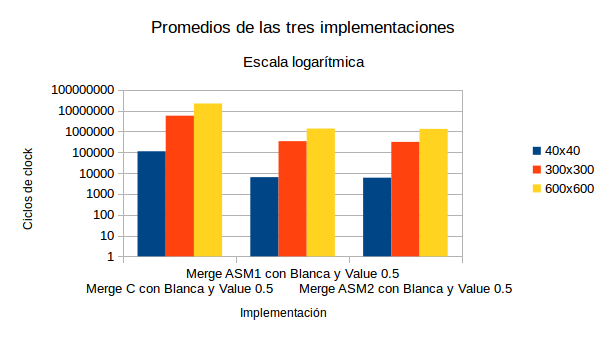
\includegraphics[width=90mm]{merge/grafico_merge_conBlancas.png}
%\caption{A simple caption \label{overflow}}
\end{figure}


Las siguientes son las tablas correspondientes a la ejecución del filtro para cada una de todas las imágenes del conjunto de casos de prueba 'mergeadas' con la imagen uniforme negra.

\begin{tabular}{| l | l | l | l | l |}
\hline
Implementación & Color & 1600 píxeles & 90000 píxeles & 360000 píxeles\\
\hline
Merge C con Negra y Value 0.5 & azul & 112601.93 &	5639322.00 &	21469172.00\\ 
\hline
Merge C con Negra y Value 0.5 & blanco & 98544.67	& 5963986.00 &	21739485.33\\ 
\hline
Merge C con Negra y Value 0.5 & mixto & 111715.11	& 5427554.33 &	21890057.78\\ 
\hline
Merge C con Negra y Value 0.5 & negro & 121468.75	& 5994952.25 &	21164423.00\\
\hline
Merge C con Negra y Value 0.5 & rojo & 109971.00	& 5852953.63	& 21210556.00\\
\hline
Merge C con Negra y Value 0.5 & verde & 106222.00 &	5679551.50	& 20684177.00\\ 
\hline
Promedio & &  110087.24	& 5759719.95 &	21359645.19\\
\hline
Desvio estándard  && 7572.28	& 217719.09	& 436854.38\\
\hline
Porcentaje de desviación  && 6.88\%	& 3.78\% &	2.05\%\\
\hline
\end{tabular}


\begin{tabular}{| l | l | l | l | l |}
\hline
Implementación & Color & 1600 píxeles & 90000 píxeles & 360000 píxeles\\
\hline
Merge ASM1 con Negra y Value 0.5 & azul & 6670.00 &	339259.67 &	1370217.47\\ 
\hline
Merge ASM1 con Negra y Value 0.5 & blanco & 7953.00 &	335490.33	& 1379671.33\\ 
\hline
Merge ASM1 con Negra y Value 0.5 & mixto & 6369.33	& 341912.22 &	1356897.33\\ 
\hline
Merge ASM1 con Negra y Value 0.5 & negro & 6424.25 &	335257.00 &	1384766.75\\
\hline
Merge ASM1 con Negra y Value 0.5 & rojo & 7097.88 &	343915.63 &	1372561.50\\
\hline
Merge ASM1 con Negra y Value 0.5 & verde & 6359.50	& 345085.00 &	1389391.00\\ 
\hline
Promedio & &  6812.33	& 340153.31 &	1375584.23\\
\hline
Desvio estándard  && 625.27	& 4197.29	& 11651.52\\
\hline
Porcentaje de desviación  && 9.18\% &	1.23\% &	0.85\%\\
\hline
\end{tabular}


\begin{tabular}{| l | l | l | l | l |}
\hline
Implementación & Color & 1600 píxeles & 90000 píxeles & 360000 píxeles\\
\hline
Merge ASM2 con Negra y Value 0.5 & azul & 5993.67	& 309772.60 & 	1292696.93\\ 
\hline
Merge ASM2 con Negra y Value 0.5 & blanco & 6841.33	& 301941.67 &	1245065.00\\ 
\hline
Merge ASM2 con Negra y Value 0.5 & mixto & 6352.22	& 309041.00	& 1343273.56\\ 
\hline
Merge ASM2 con Negra y Value 0.5 & negro & 6628.00	& 320615.50	& 1338728.00\\
\hline
Merge ASM2 con Negra y Value 0.5 & rojo & 6009.38	& 305238.13	& 1357228.63\\
\hline
Merge ASM2 con Negra y Value 0.5 & verde & 6338.00	& 312857.75	& 1279955.25\\ 
\hline
Promedio & &  6360.43	& 309911.11	& 1309491.23\\
\hline
Desvio estándard  && 335.02	& 6471.35	& 43772.26\\
\hline
Porcentaje de desviación  && 5.27\% &	2.09\% &	3.34\%\\
\hline
\end{tabular}

Como en las secciones anteriores, tomando los promedios para cada tamaño, en cada implementación, podemos ilustrar la performance de las distints implementaciones en el gráfico que sigue.

\begin{tabular}{| l | l | l | l|}
\hline
Implementación  & 1600 píxeles & 90000 píxeles & 360000 píxeles\\
\hline
Merge C con Negra y Value 0.5  & 110087.24	& 5759719.95	& 21359645.19\\
\hline
Merge ASM1 con Negra y Value 0.5  & 6812.33 &	340153.31	& 1375584.23\\
\hline
Merge ASM2 con Negra y Value 0.5 & 6360.43	& 309911.11	& 1309491.23\\
\hline
\end{tabular}

\begin{figure}[ht]
\centering
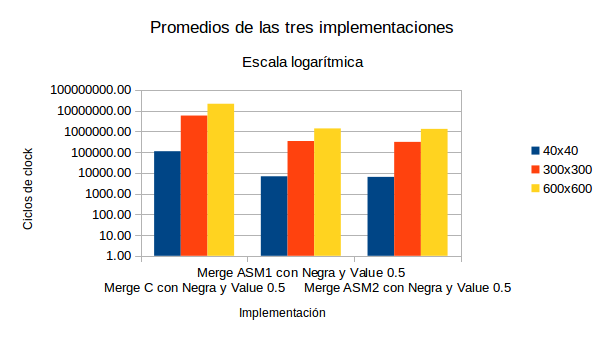
\includegraphics[width=90mm]{merge/grafico_merge_conNegras.png}
%\caption{A simple caption \label{overflow}}
\end{figure}

\subsubsection{Algunas conclusiones}
Para este filtro, la implementación más rápida es ASM2.\\
Como en los otros filtros, el tamaño de la imágen es un factor que incide en los ciclos de clock que demora la ejecución de una implementación, siendo la evolución creciente.\\
No notamos que haya diferencias respecto de los tipos de imágenes utilizados, ya que para cada implementación, si miramos la fila que calcula los porcentajes de desvío estándard entre los distintos subgrupos de imágenes, veremos que los porcentajes son pequeños y de esta forma, ninguna implementación se desvía significativamente del promedio.\\
Tampoco notamos diferencias notables entre los casos de pruebas en los que se 'mergeó' con la imagen uniforme blanca, respecto de los que se 'mergeó' con la imagen uniforme negra. De este modo, el tipo de imagen a ser 'mergeada' tampoco parece ser el factor de incidencia en la performance de este filtro.\\
Si bien la diferencia de tiempo de ejecución de ASM1 y ASM2 no es marcada, como mencionamos anteriormente ASM2 resulta ser la implementación más performante. Lo que la diferencia de la otra implementación de Assembler es justamente que ASM2 realiza todas las operaciones en enteros y que no debe realizar las -costosas- operaciones de conversión a punto flotante y luego de punto flotante a enteros que realiza en cada iteración del ciclo ASM1. Dado que la cantidad de operaciones en ambas implementaciones es similar, creemos que las anteriores cuestiones son las determinantes para que ASM2 sea la implementación más rápida para este filtro.\\



% Fin Merge

\newpage	
% Comienzo HSL
\section{HSL}
\subsection{Introducción}
\textit{HSL} es un filtro que consta de tres etapas:
\begin{enumerate}
\item \textbf{RGBtoHSL:} consiste en un cambio del espacio de color de los píxeles, desde RGB a HSL. 
\item \textbf{Suma:} se procesan los píxeles sumándole valores pasados por parámetro a cada una de las componentes.
\item \textbf{RGBtoHSL:} se realiza la operación inversa a la de la primera etapa, es decir, el pasaje del espacio HSL a RGB.
\end{enumerate}

El pseudocódigo de cada una de estas etapas es descripto en el enunciado del TP.

\subsection{Implementación 1}
En esta sección se pide realizar una implementación de la etapa de \textit{Suma} en ASM y desde la misma llamar a las funciones en C para convertir entre RGB y HSL.\\
Como las funciones \textit{RGBtoHSL} y \textit{HSLtoRGB} procesan de a un píxel, es necesario iterar sobre cada píxel de la imagen para ir realizando las conversiones y procesándolos.\\

De esta forma, los pasos que se realizan en una iteración del ciclo son los siguientes:

\begin{enumerate}

\item Tomar un píxel de la imagen.
\item Llamar a la función \textit{RGBtoHSL} de C.
\item Con el píxel ya transformado al espacio HSL, hay que realizar la operación de suma en sí. Esta se realiza de la siguiente manera:\\

\textbf{Pseudocódigo de Suma}
\begin{verbatim}
	if( h+HH >= 360 ) h = h + HH - 360
	else if( h+HH < 0 ) h = h + HH + 360
	else
	    h = h + HH
	if( s+SS >= 1 ) s = 1
	else if( s+SS < 0 ) s = 0
	else
	    s = s + SS
	if( l+LL >= 1 ) l = 1
	else if( l+LL < 0 ) l = 0
	else
	    l = l + LL         
\end{verbatim}
Para poder realizar estas operaciones, necesitamos armar un registro de que contenga cuatro dwords que tengan la siguiente forma:

\begin{tabular}{| g | g | g | g |} %tabla color orange
\hline
$l+LL$ & $s+SS$ & $h+HH$ & $aa$ \\ 
\hline
\end{tabular}

Donde \textit{h}, \textit{s} y \textit{l} son las componentes del píxel HSL y \textit{HH}, \textit{SS} y \textit{LL} los valores pasados como parámetros. El \textit{aa} es el dword correspondiente al alfa, que va a quedar sin modificaciones.

Para realizar el registro mostrado anteriormente realizamos las siguientes operaciones:

\begin{lstlisting}
movss xmm1, [posicion_de_memoria_donde_esta_LL]	;xmm1 = |00|00|00|LL|
pslldq xmm1, 12			;xmm1 = |00|00|LL|00| - shift a izquierda
movss xmm2, [posicion_de_memoria_donde_esta_SS]	;xmm1 = |00|00|LL|SS|
pslldq xmm2, 8			;xmm1 = |00|LL|SS|00| - shift a izquierda
movss xmm3, [posicion_de_memoria_donde_esta_HH]	;xmm1 = |00|LL|SS|HH|
pslldq xmm3, 4			;xmm1 = |LL|SS|HH|aa| - shift a izquierda
\end{lstlisting}
Y luego, sumamos este registro al registro en donde tenemos a los tres componentes HSL de píxel.\\ Llamaremos a este registro \textit{origen} para claridad.

Estas operaciones debemos realizarlas en cada iteración del ciclo, porque tras el llamado a funciones de C, la convención no nos asegura que los registros XMM mantendrán sus valores.\\
Por último en este paso, vamos a armar las máscaras que necesitamos para realizar las operaciones del pseudocódigo que mostramos al principio de este punto.\\
Realizamos los siguientes defines:\\
\begin{verbatim}
comparar: dd 0.0, 360.0, 1.0, 1.0
vuelta_atras: dd 0.0, -360.0, 1.0, 1.0
vuelta_adelante: dd	0.0, 360.0, 0.0, 0.0         
\end{verbatim}
Y preparamos los siguientes registros:
\begin{lstlisting}
;traigo mascaras
	movups xmm10, [comparar]
	pxor xmm11, xmm11	;llamaremos ceros a xmm11
	movups xmm2, [vuelta_atras]
	movups xmm3, [vuelta_adelante]

;preparo datos con mascaras
	pxor xmm5, xmm5
	movlhps xmm5, xmm0	;xmm5 = |h+HH|aa|00|00|
	psrldq xmm5, 8			;xmm5 = |00|00|h+HH|aa|
	movups xmm6, xmm5		;xmm6 = |00|00|h+HH|aa|
	addps xmm5, xmm2		;xmm5 = |1|1|h+HH-360|aa| - llamaremos resultadoTRUEif a xmm5
	addps xmm6, xmm3		;xmm6 = |0|0|h+HH+360|aa| - llamaremos resultadoFALSEif a xmm6

\end{lstlisting}

\item En el punto anterior preparamos todos los registros necesarios para finalmente en este punto, realizar la lógica de suma según el pseudocódigo visto.\\
Como las componentes están enpaquetadas, debemos realizar las comparaciones simultáneamente. Para esto nos valemos de las máscaras que realizamos anteriormente. Para claridad al mostrar al código, reemplazaremos los registros efectivamente usados por los nombres de las etiquetas definidas en los defines y en los comentarios hechos anteriormente, donde armamos las máscaras necesarias.

\begin{lstlisting}
//xmm0, xmm1, xmm7 y xmm8 son copias de origen.
;if h+HH>=360 || s+SS>1 || l+LL>1
	cmpps xmm0, comparar, 5	;5 = greater equal
	pand xmm0, resultadoTRUEif

;if 0<=h+HH<360 || 0<=s+SS<1 || 0<=l+LL<1
	cmpps xmm7, comparar, 1	;1 = less than
	cmpps xmm8, ceros, 5	;5 = greater equal - ceros es un registro con ceros hecho con un pxor entre un registro XMM y si mismo.
	pand xmm7, xmm8
	pand xmm7, xmm1

;if h+HH<0 || s+SS<0 || l+LL<0
	cmpps xmm1,	xmm11, 1	;1 = less than
	pand xmm1, resultadoFALSEif

;sumo todos los valores con las mascaras aplicadas
	por xmm0, xmm7
	por xmm0, xmm1
\end{lstlisting}
En este punto tenemos en xmm0 el resultado para cada componente tras realizar las comparaciones indicadas por el pseudocódigo y asignar el valor indicado en cada caso. 
\item Con el píxel ya modificado en todas sus componentes, ahora ya podemos pasarselo a la función \textbf{hslTOrgb} para volver a pasar al espacio RGB.
\item Finalmente, avanzamos un píxel y volvemos a iterar.

\end{enumerate}

\subsection{Implementación 2}
La consigna en esta implementación es desarrollar todas las etapas del filtro en lenguaje ensamblador.\\
De esta manera, para la etapa de \textit{Suma} se aprovechó la implementación anterior y se desarrollaron las dos etapas restantes. Es decir, ahora tendremos la conversión de RGB a HSL y de HSL a RGB en dos rutinas separadas, programadas en Assembler.\\

Al igual que en la primer implementación, se procesó de a un píxel por vez. Esto es debido a que como la etapa de suma es la misma que en la primer implementación, dicha etapa va convirtiendo de a un píxel así que se respetó esa forma de trabajo.\\

\underline{\textbf{Nota 1:}} Para realizar todas las comparaciónes, (los \textbf{ifs}) se uso la instrucción \textbf{cmpps}, la cual, dado un modo de comparación, aplica en el operando destino, una máscara con los valores resultantes de la comparación, grabando todas Fs si el resultado es \textit{true} y todos 0s si el resultado es \textit{false}

\underline{\textbf{Nota 2:}} Para el cálculo de \textbf{fabs} lo que se hizo fue simplemente cambiar el valor del bit más significativo a 0, ya que en la representación de floats, ese es el bit que indica el signo del float; para realizar esto, se hizo AND bit a bit con una mascara que contenía todos 1s, excepto en el bit más significativo que tenía un 0.

\underline{\textbf{Nota 3:}} Para el cálculo de \textbf{fmod} lo que se hizo fue aplicar el calculo de fmod, el cual es:
\begin{verbatim}
	fmod = numerador - tquot * denominador
	donde tquot es el resultado (truncado a 0) de numerador/denominador
\end{verbatim}
Para realizar ese cálculo de hizo uso de las instrucciones \textbf{divss} y \textbf{roundss}.\\
Fuente: http://www.cplusplus.com/reference/cmath/fmod/ \\\\

Para la \textbf{primer conversión} (\textit{RGB to HSL}) se busca a mano el máximo y mínimo de las componentes. Una vez con dichos valores calculados, ya podemos comenzar a definir los valores de $H$, $S$ y $L$.\\
También se obtuvo el valor de $d$ via la resta del máximo menos el mínimo, necesario para el cálculo de $H$ y $S$.\\



\textbf{Cálculo de H}\\
Para definir $H$ se evaluaron los distintos casos posibles:
donde la componente mínima era igual a la máxima, y donde la máxima era o bien igual a R, o bien igual a G o bien igual a B. En cada uno se realizo el proceso correspondiente indicado en el enunciado del trabajo, el cual dicta:

\begin{verbatim}
	if( cmax == cmin ) h = 0
	else if( cmax == r ) h = 60 * ((g-b)/d + 6)
	else if( cmax == g ) h = 60 * ((b-r)/d + 2)
	else if( cmax == b ) h = 60 * ((r-g)/d + 4)
	    
	if( h >= 360 ) h = h - 360

\end{verbatim}

\textbf{Cálculo de L}\\
Luego para el calculo de $L$, se realizó la cuenta especificada en el enunciado:

\begin{verbatim}
	l = ( cmax + cmin ) / 510

\end{verbatim}

\textbf{Cálculo de S}\\
Y por último, para el valor de $S$, se realizó el siguiente chequeo y la asignación correspondiente, tal como dicta el enunciado:

\begin{verbatim}
	if ( cmax == cmin )
	    s = 0
	else
	    s = d / ( 1 - fabs( 2*l - 1 ) ) / 255.0001f;

\end{verbatim}

\newpage
Para la \textbf{segunda conversión} (\textit{HSL to RGB}), primero se computó el valor de $c$, $x$ y $m$. Para conseguir esas 3 variables, se realizaron los siguientes calculos dados en el enunciado del TP:

\begin{verbatim}
	c = ( 1 - fabs( 2*l - 1 )) * s;
	x = c * ( 1 - fabs( fmod( h/60, 2 ) - 1 ) )
	m = l - c / 2
\end{verbatim}
El cálculo de \textbf{fabs} y \textbf{fmod} fueorn calculados como se describió en las notas 2 y 3 anteriores.\\

Luego, se procedió a realizar el cálculo de $R$, $G$ y $B$, evaluando los siguientes 6 casos en donde h puede oscilar:

\begin{verbatim}
	if(   0<=h && h<60  ) r=c b=x g=0
	if(  60<=h && h<120 ) r=x b=c g=0
	if( 120<=h && h<180 ) r=0 b=c g=x
	if( 180<=h && h<240 ) r=0 b=x g=c
	if( 240<=h && h<300 ) r=x b=0 g=c
	if( 300<=h && h<360 ) r=c b=0 g=x
\end{verbatim}
Para esto se uso la instrucción cmpss y algo de logica para hacer los distintos "ifs" necesarios tal como se declara en la \textbf{nota 1}.\\


Casi terminando, se hace el calculo de la escala, mediante las siguientes sumas y multiplicaciones:
\begin{verbatim}
r = (r+m) * 255
g = (g+m) * 255
b = (b+m) * 255
\end{verbatim}
Para las mismas, se hizo uso de la instrucciones \textbf{addss} y \textbf{mulps}.\\


Finalmente, hacemos uso de la instrucción \textbf{cvtss2si} para convertir los valores de R, G y B a enteros.

Este último paso nos da finalmente los valores de RGB para devolver. (La componente de transparencia, no se tiene en cuenta para la explicación ya que no tiene lógica de procesado, simplemente se la transforma de float a entero y se devuelve.)\\
Estos mismos los cargamos en el puntero a \textit{uint8\_t} pasado por parámetro y se retorna a la rutina principal.\\

\subsection{Resultados}
A continuación, mostraremos algunos de los resultados y conclusiones a los cuales llegamos a través de la experimentación de las distintas implementaciones según la estretegia ideada para este fin, detallada en la introducción.

Tener en cuenta que el porcentaje de desvío estándard para cada implementación de este filtro resultó ser de:
\begin{tabular}{| l | l |}
\hline
Implementación & Porcentaje de Desvío Estándard \\
HSL C	& $+/- 3\%$\\
HSL ASM1 & 	$+/- 6\%$\\
HSL ASM2	& $+/- 5\%$\\
\hline
\end{tabular}

Estos porcentajes representan que, para cada medición de cantidad de ciclos de clock de ejecución de una implementación dada de este filtro, tras descartar el 10\% de las peores mediciones, y tomar el promedio entre el 90\% de las mediciones restantes, el error varía entre +/- dicho porcentaje. Por ejemplo, dada la ejecución siguiente:

\begin{verbatim}
c hsl image_1_40x40.bmp salida.bmp 0.5 0.5 0.5
\end{verbatim}
Sobre las 100 repeticiones realizadas, tras descartar el 10\% de las peores, quedan 90 mediciones sobre las cuales el promedio calculado fue 209670 con margen de error de +/-3\%.\\

Las tablas a continuación representan, para cada implementación el promedio para las imágenes tendientes a un color determinado en cada uno de los distintos tamaños testeados. A su vez, en las últimas tres filas, se calcula el promedio general para dichos promedios, el desvío estandar entre ellos y el porcentaje de desvío.

\begin{tabular}{| l | l | l | l | l |}
\hline
Implementación & Color & 1600 píxeles & 90000 píxeles & 360000 píxeles\\
\hline
Hsl ASM1 0.5 0.5 0.5 & azul & 359764.53 & 18520763.60 & 72633855.47\\ 
\hline
Hsl ASM1 0.5 0.5 0.5 & blanco & 310855.33 & 18855768.67 & 70170817.33\\ 
\hline
Hsl ASM1 0.5 0.5 0.5 & mixto & 327535.44 & 18280896.22 & 72698313.33\\ 
\hline
Hsl ASM1 0.5 0.5 0.5 & negro & 223275.25 & 12070519.50 & 49497420.00\\
\hline
Hsl ASM1 0.5 0.5 0.5 & rojo & 329826.75 & 17855115.50 & 69956707.00\\
\hline
Hsl ASM1 0.5 0.5 0.5 & verde & 315792.50 & 18595604.50 & 71852216.00\\ 
\hline
Promedio & &  311174.97 & 17363111.33 & 67801554.86\\
\hline
Desvio estándard  && 46312.60 & 2614695.00  & 9044740.65\\
\hline
Porcentaje de desviación  && 14.88\% & 15.06\% & 13.34\%\\
\hline
\end{tabular}

\begin{tabular}{| l | l | l | l | l |}
\hline
Implementación & Color & 1600 píxeles & 90000 píxeles & 360000 píxeles\\
\hline
Hsl ASM2 0.5 0.5 0.5 & azul & 284234.93 & 12611483.33 & 50635606.13\\ 
\hline
Hsl ASM2 0.5 0.5 0.5 & blanco & 284863.67 & 13172857.33 & 50869777.33\\ 
\hline
Hsl ASM2 0.5 0.5 0.5 & mixto & 282192.78 & 13088796.78 & 50706775.56\\ 
\hline
Hsl ASM2 0.5 0.5 0.5 & negro & 233569.25 & 10897850.25 & 42586066.00\\
\hline
Hsl ASM2 0.5 0.5 0.5 & rojo & 291041.13 & 12736569.25 & 51346788.00\\
\hline
Hsl ASM2 0.5 0.5 0.5 & verde & 290393.00 & 12734652.00 & 51201397.00\\ 
\hline
Promedio & &  277715.79 & 12540368.16 & 49557735.00\\
\hline
Desvio estándard  &&  21912.68 & 834263.75 & 3426661.92\\
\hline
Porcentaje de desviación  &&  7.89\% &  6.65\% &  6.91\%\\
\hline
\end{tabular}

\begin{tabular}{| l | l | l | l | l |}
\hline
Implementación & Color & 1600 píxeles & 90000 píxeles & 360000 píxeles\\
\hline
Hsl C 0.5 0.5 0.5 & azul &  365585.53 & 16842125.00 & 64348957.33\\ 
\hline
Hsl C 0.5 0.5 0.5 & blanco & 377779.67 & 16876860.00 & 64668644.00\\ 
\hline
Hsl C 0.5 0.5 0.5 & mixto & 334989.89 & 16393089.44 & 64292180.89\\ 
\hline
Hsl C 0.5 0.5 0.5 & negro & 276944.25 & 11694642.25 & 46741104.00\\
\hline
Hsl C 0.5 0.5 0.5 & rojo &  350354.38 & 15877406.88 & 62859643.00\\
\hline
Hsl C 0.5 0.5 0.5 & verde &  360322.75 & 15394790.00 & 63306250.00\\ 
\hline
Promedio & &  344329.41 & 15513152.26 & 61036129.87\\
\hline
Desvio estándard  &&  36030.03  & 1955907.29 & 7037020.15\\
\hline
Porcentaje de desviación  && 10.46\% & 12.61\% &  11.53\%\\
\hline
\end{tabular}

A partir de éstas, confeccionamos la siguiente tabla que luego graficamos, utilizando escala logarítmica, para poder evaluar cómo era el rendimiento en promedio de las tres implementaciones en los distintos tamaños de imágenes.\\

\begin{tabular}{| l | l | l | l|}
\hline
Implementación	& 1600 píxeles & 90000 píxeles & 360000 píxeles\\
\hline
Hsl ASM1 0.5 0.5 0.5	& 311174.96	& 17363111.33 & 	67801554.85\\
\hline
Hsl ASM2 0.5 0.5 0.5	& 277715.79	& 12540368.15	& 49557735.00\\
\hline
Hsl C 0.5 0.5 0.5	& 344329.41	& 15513152.26	& 61036129.87\\
\hline
\end{tabular}

\begin{figure}[ht]
\centering
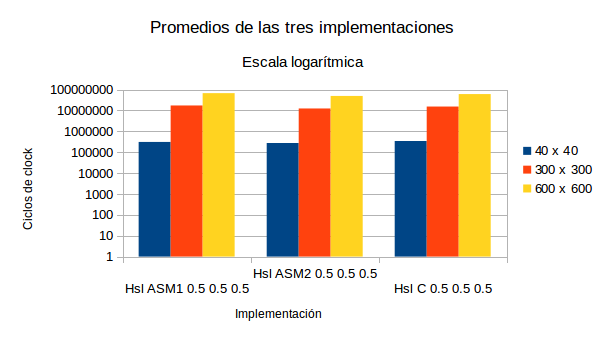
\includegraphics[width=90mm]{hsl/graficoHsl.png}
%\caption{A simple caption \label{overflow}}
\end{figure}

A continuación, mostraremos las tablas correspondientes a las imágenes de tipo "color constante", es decir, imágenes puramente rojas, verdes, azules, blancas y negras, que tratamos por separado para evaluar si registraban un comportamineto distinto.\\

\begin{tabular}{| l | l | l | l | l |}
\hline
Implementación & Color & 1600 píxeles & 90000 píxeles & 360000 píxeles\\
\hline
Hsl ASM1 0.5 0.5 0.5 & Uniforme Blanca & 231075.00 & 10941995.00 & 41332836.00\\ 
\hline
Hsl ASM1 0.5 0.5 0.5 & Uniforme Negra & 233186.00 & 13472777.00 & 45535360.00\\ 
\hline
Hsl ASM1 0.5 0.5 0.5 & Uniforme Roja & 419964.00 & 18202474.00 & 74076088.00\\ 
\hline
Hsl ASM1 0.5 0.5 0.5 & Uniforme Verde & 392571.00 & 17789276.00 & 71168984.00\\
\hline
Hsl ASM1 0.5 0.5 0.5 & Uniforme Azul & 359244.00 & 17842096.00 & 72150072.00\\
\hline
Promedio & &  327208.00	& 15649723.60 & 60852668.00\\
\hline
Desvio estándard  &&  89420.35 & 3271181.78 & 16004376.86\\
\hline
Porcentaje de desviación  &&  27.33\% & 20.90\% & 26.30\%\\
\hline
\end{tabular}

\begin{tabular}{| l | l | l | l | l |}
\hline
Implementación & Color & 1600 píxeles & 90000 píxeles & 360000 píxeles\\
\hline
Hsl ASM2 0.5 0.5 0.5 & Uniforme Blanca & 261370.00 & 11202093.00 & 41456304.00\\ 
\hline
Hsl ASM2 0.5 0.5 0.5 & Uniforme Negra & 200118.00 & 10637117.00	& 40151872.00\\ 
\hline
Hsl ASM2 0.5 0.5 0.5 & Uniforme Roja & 09031.00	& 13109446.00 & 53225056.00\\ 
\hline
Hsl ASM2 0.5 0.5 0.5 & Uniforme Verde & 305518.00 & 12530113.00	& 51572832.00\\
\hline
Hsl ASM2 0.5 0.5 0.5 & Uniforme Azul & 292952.00 & 12556929.00 & 50722960.00\\
\hline
Promedio & &  273797.80	& 12007139.60 & 47425804.80\\
\hline
Desvio estándard  &&  45270.29	& 1038738.53	& 6128731.92\\
\hline
Porcentaje de desviación  &&  16.53\% & 	8.65\% & 	12.92\%\\
\hline
\end{tabular}

\begin{tabular}{| l | l | l | l | l |}
\hline
Implementación & Color & 1600 píxeles & 90000 píxeles & 360000 píxeles\\
\hline
Hsl C 0.5 0.5 0.5 & Uniforme Blanca & 204029.00	& 10340318.00 & 39518652.00\\ 
\hline
Hsl C 0.5 0.5 0.5 & Uniforme Negra & 233486.00	& 10644786.00 &	40521400.\\ 
\hline
Hsl C 0.5 0.5 0.5 & Uniforme Roja & 356866.00	& 16543328.00	& 63436016.00\\ 
\hline
Hsl C 0.5 0.5 0.5 & Uniforme Verde & 354434.00	& 15911884.00	& 62773144.00\\
\hline
Hsl C 0.5 0.5 0.5 & Uniforme Azul & 343594.00	& 16214899.00	& 61588924.00\\
\hline
Promedio & &  298481.80	& 13931043.00	& 53567627.20\\
\hline
Desvio estándard  &&  73688.97	& 3148672.47	& 12389971.63\\
\hline
Porcentaje de desviación  &&  24.69\%	& 22.60\% & 23.13\%\\
\hline
\end{tabular}

De manera análoga, tomando los promedios obtenidos, graficamos para poder comparar las performances de las implementaciones en estos casos.\\

\begin{tabular}{| l | l | l | l|}
\hline
Implementación	& 1600 píxeles & 90000 píxeles & 360000 píxeles\\
\hline
Hsl ASM1 0.5 0.5 0.5	& 327208	& 15649723.6	& 60852668\\
\hline
Hsl ASM2 0.5 0.5 0.5	&273797.8	& 12007139.6	& 47425804.8\\
\hline
Hsl C 0.5 0.5 0.5	& 298481.8	& 13931043	& 53567627.2\\
\hline
\end{tabular}


\begin{figure}[ht]
\centering
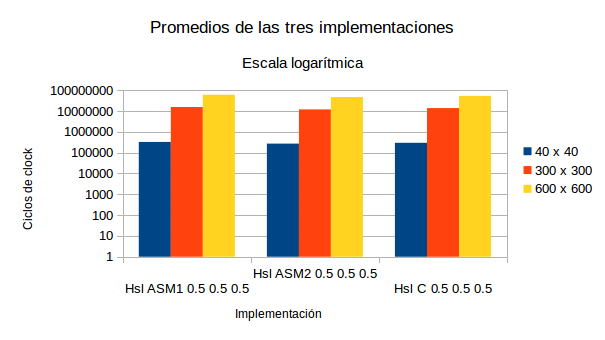
\includegraphics[width=90mm]{hsl/graficoHsl_cte.png}
%\caption{A simple caption \label{overflow}}
\end{figure}

\subsubsection{Algunas conclusiones}
Para HSL, la implementación más performante para los tres tamaños propuestos es ASM2, de la misma manera en que resultó ser para los otros filtros.\\
Dentro de cada implementación, como en los casos anteriores, los tiempos de ejecución evolucionan de manera creciente a medida que aumenta la cantidad de píxeles en las imágenes; totalmente esperable.\\

Sin embargo, y tomando como estrategia de medición respecto de las diferencias entre los distintos tipos de imágenes la misma que la detallada en la introducción, los porcentajes de desvío estándar es mayor que en los otros filtros. Este resultado es en parte el esperado, ya que en esta implementación se toman acciones diferentes según el resultado que da sumar el color del píxel de la imagen al del parámetro recibido, entonces, es esperable que los tiempos de implementación divergieran en función de los distintos tipos de imágenes que tienden a distintos colores.\\

Sin tener en cuenta que las diferencias de performance en las distintas implementaciones de este ciclo se ven relacionadas con el uso de C o Assembler (en los distintos filtros se usa, o bien todo C, o bien mixto -implementación ASM1- o bien todo Assembler -en ASM2-), el punto anterior referente a la diferencia entre los tipos de imágenes es el más llamativo a la hora de evaluar la performance de las distintas implementaciones, a diferencia tal vez de los otros filtros implementados, en donde la desviación estándar en función de los tipos de imágenes era significativamente menor. 
% Fin HSL

\end{document}